%!TEX root = ../documentation.tex
\chapter{Models}
\label{ch:models}

Da es in der Regel nicht \textit{das} Perfekte Modell gibt um Klassen zu klassifizieren, haben wir hier verschiedene verglichen. Dabei haben wir uns hauptsächlich auf ResNet und SqueezeNet konzentriert, da diese beiden Modelle Erfahrungsgemäß, laut anderen Berichten, die höchste Accuracy hatten.
Damit man diese Netze jedoch nutzen kann, muss man erstmal wissen, wie genau sie funktionieren.

\section{ResNet152}

ResNet ist eine der beliebtesten CNN Architekturen, dadurch, dass es der Sieger der ImageNet competition in 2015 war. ResNet bietet einen einfachen \textit{gradient flow} für noch effizienteres Training.
\newline Die Hauptidee bei ResNet ist es einige Layers gezielt zu überspringen. Hierdurch kann das Netz einen direkten Weg zu den ersten layern aufbauen wodurch die gradient updates für diese Layer vereinfacht werden. Zudem gibt es verschiedene Versionen von ResNet, welche alle jedoch sehr ähnlich sind, sich nur in der Anzahl der Layer unterscheiden (ResNet18, ResNet50, ResNet152,..).
Dieses Modell wird in der folgenden Abbildung presäntiert(Als ResNet18 Version), muss dann jedoch mit anderen Modellen verglichen werden, um vorallem auch Faktoren wie Parameter etc. zu anzupassen.

\begin{figure}[H]
    \centering
    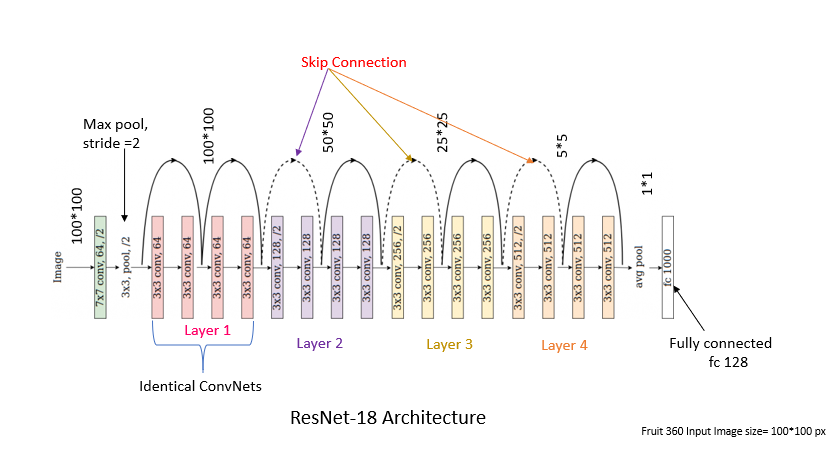
\includegraphics[width=1.1\textwidth]{Bilder/ResNet18Model.png}
    \caption{}
    \label{fig:ResNet18}
\end{figure}

\section{SqueezeNet}

SqueezeNet ist eine CNN Architektur und erreicht AlexNet-Genauigkeit auf ImageNet, mit 50x weniger Parametern. Mit zusätzlichen Funktionen zur Modell-Kompression, lässt sich SqueezeNet zudem auf weniger als 0.5MB verkleinern, somit 510x kleiner als AlexNet.
\newline Hierbei wird zu einem 1x1 Layer gewechselt, welches den Input in der vertikalen Dimension komprimiert, daher der Name \textit{squeeze}, gefolgt von insgesamt zwei paralellen 1x1 und 3x3 convolutional layern, wodurch die Tiefe der Daten wieder erweitert wird.
\newline Das Modell ist hierdurch klar, jedoch muss das komprimieren der Parameter genauer angeschaut werden, da es hierfür drei verschiedene Strategien gibt. Die erste hierbei ist 3x3 Filter durch 1x1 Filter auszutauschen, da ein 3x3 Filter 9x so viele Parameter hat wie ein 1x1 Filter. Als zweite Strategie wird die Anzahl der Eingabe-Kanäle, zu den 3x3 Filtern, reduziert. Da die Anzahl der Parameter wie folgt berechent wird: 
\newline (Anzahl der Eingabe-Kanäle) * (Anzahl der Filter) * (3*3)
Einen Faktor haben wir durch Strategie 1 bereits reduziert, bei Strategie 2 reduziert man somit einen weiteren Faktor, um somit das insgesamte Produkt der Parameter zu reduzieren. Hierbei werden oft \textit{squeeze layers} benutzt um die Anzahl der Eingabe-Kanäle zu reduzieren. Zuletzt die dritte Strategie, die verwendet wird, ist das späte \textit{downsample} im Netz, so dass die Convolution Layers große \textit{activation maps} haben. Da in einem Convolutional Netz jedes Convolution Layer ein \textit{output activation map} erzeugt, welche 1x1 oder größer ist und durch die größe der Eingabedaten der Wahl der layers bestimmt wird, werden diese durch \textit{downsample}, in der CNN Architektur, verkleinert. In der Folgenden Abbildung wird Architektur veranschaulicht.

\begin{figure}[H]
    \centering
    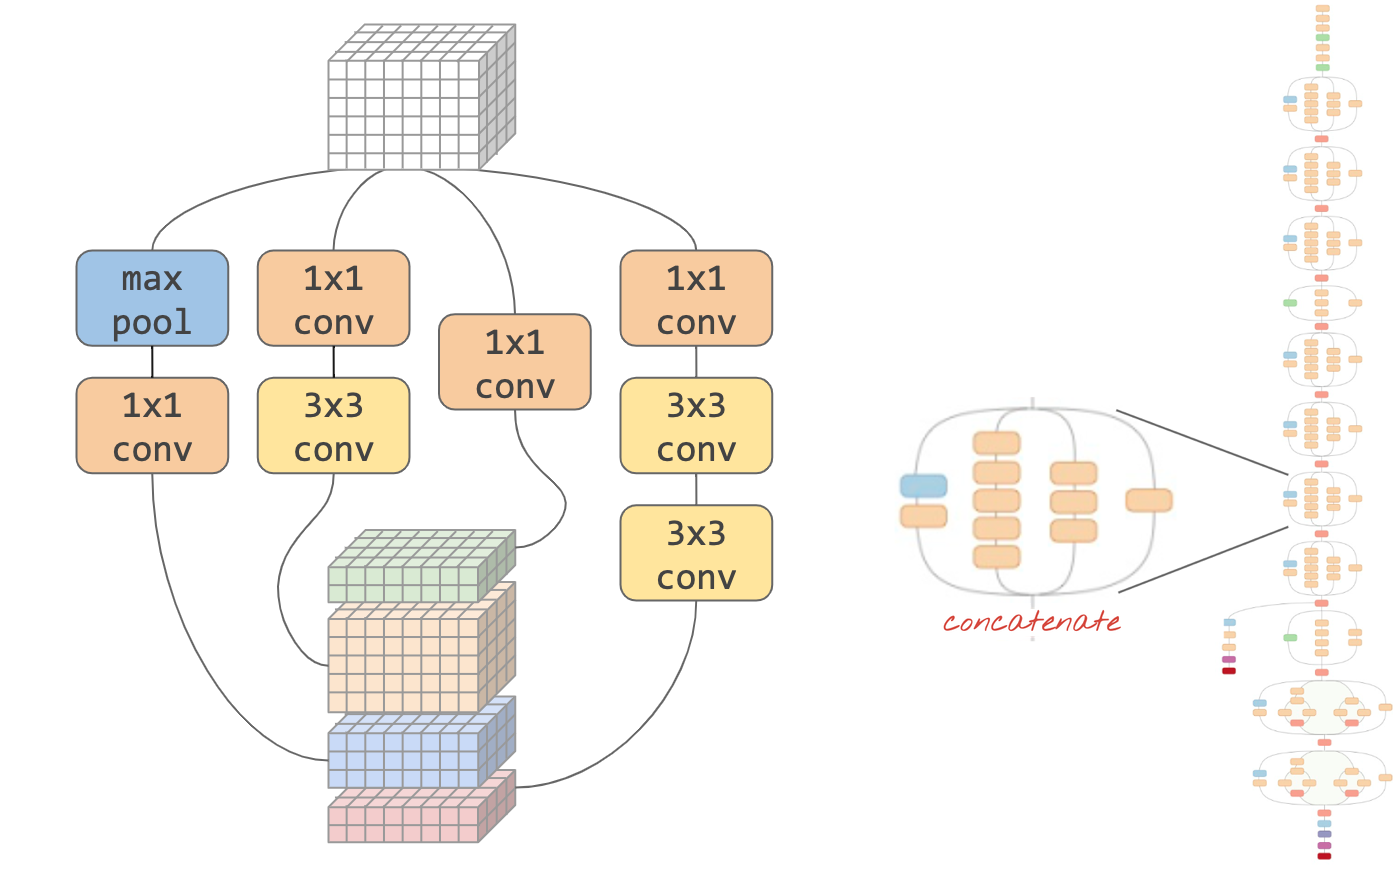
\includegraphics[width=0.82\textwidth]{Bilder/SqueezeNetModel.png}
    \caption{SqueezeNet}
    \label{fig:SqueezeNet}
\end{figure}
